\documentclass[mstat,12pt]{unswthesis}


\newlength{\cslhangindent}
\setlength{\cslhangindent}{1.5em}
\newenvironment{CSLReferences}%
  {}%
  {\par}

\usepackage{pgfgantt}

\usepackage{float}
\usepackage[a4paper, margin=1in]{geometry}
\usepackage{booktabs}
\usepackage{tabularx}
\usepackage{rotating}
\usepackage{enumitem}
\usepackage{pdflscape}
\usepackage{geometry}
\usepackage{caption}[hypcap=false]
\captionsetup[table]{skip=10pt}

\usepackage{catchfile}
\usepackage[section, nottoc]{tocbibind}

% Custom column type to vertically center cell content
\newcolumntype{M}[1]{>{\centering\arraybackslash}m{#1}}
\newcolumntype{Y}{>{\centering\arraybackslash}X}


%%%%%%%%%%%%%%%%%%%%%%%%%%%%%%%%%%%%%%%%%%%%%%%%%%%%%%%%%%%%%%%%%%
% 
% OK...Now we get to some actual input.  The first part sets up
% the title etc that will appear on the front page
%
%%%%%%%%%%%%%%%%%%%%%%%%%%%%%%%%%%%%%%%%%%%%%%%%%%%%%%%%%%%%%%%%%

\title{Group Project Plan by Team K\\[0.5cm]}

\authornameonly{Doug Smithers (z5135363), Tom Bernstein (z3478832), Daniel Sartor (z5350306). }

\author{\Authornameonly}

\copyrightfalse
\figurespagefalse
\tablespagefalse

%%%%%%%%%%%%%%%%%%%%%%%%%%%%%%%%%%%%%%%%%%%%%%%%%%%%%%%%%%%%%%%%%
%
%  And now the document begins
%  The \beforepreface and \afterpreface commands puts the
%  contents page etc in
%
%%%%%%%%%%%%%%%%%%%%%%%%%%%%%%%%%%%%%%%%%%%%%%%%%%%%%%%%%%%%%%%%%%


%%%%%%%%%%%%%%%%%%%%%%%%%%%%%%%%%%%%%%%%%%%%%%%%%%%%%%%%%%%%%%%%%%%%%%%
%
%  A small sample UNSW Coursework Masters thesis file.
%  Any questions to Ian Doust i.doust@unsw.edu.au and/or Gery Geenens ggeenens@unsw.edu.au
%
%%%%%%%%%%%%%%%%%%%%%%%%%%%%%%%%%%%%%%%%%%%%%%%%%%%%%%%%%%%%%%%%%%%%%%%
%
%  The first part pulls in a UNSW Thesis class file.  This one is
%  slightly nonstandard and has been set up to do a couple of
%  things automatically
%
 
%%%%%%%%%%%%%%%%%
%% Precisely one of the next four lines should be uncommented.
%% Choose the one which matches your degree, uncomment it, and comment out the other two!
%\documentclass[mfin,12pt]{unswthesis}    %%  For Master of Financial Mathematics 
%\documentclass[mmath,12pt]{unswthesis}   %%  For Master of Mathematics
%\documentclass[mstat,12pt]{unswthesis}  %%  For Master of Statistics
%%%%%%%%%%%%%%%%%



\linespread{1}
\usepackage{amsfonts}
\usepackage{amssymb}
\usepackage{amsthm}
\usepackage{latexsym,amsmath}
\usepackage{graphicx}
\usepackage{afterpage}
\usepackage[colorlinks]{hyperref}
 \hypersetup{
     colorlinks=true,
     linkcolor=blue,
     filecolor=blue,
     citecolor= black,      
     urlcolor=cyan,
     }
\usepackage{textcomp}
\usepackage{longtable}
\usepackage{booktabs}
\usepackage{float}

%%%%%%%%%%%%%%%%%%%%%%%%%%%%%%%%%%%%%%%%%%%%%%%%%%%%%%%%%%%%%%%%%
%
%  The following are some simple LaTeX macros to give some
%  commonly used letters in funny fonts. You may need more or less of
%  these
%
\newcommand{\R}{\mathbb{R}}
\newcommand{\Q}{\mathbb{Q}}
\newcommand{\C}{\mathbb{C}}
\newcommand{\N}{\mathbb{N}}
\newcommand{\F}{\mathbb{F}}
\newcommand{\PP}{\mathbb{P}}
\newcommand{\T}{\mathbb{T}}
\newcommand{\Z}{\mathbb{Z}}
\newcommand{\B}{\mathfrak{B}}
\newcommand{\BB}{\mathcal{B}}
\newcommand{\M}{\mathfrak{M}}
\newcommand{\X}{\mathfrak{X}}
\newcommand{\Y}{\mathfrak{Y}}
\newcommand{\CC}{\mathcal{C}}
\newcommand{\E}{\mathbb{E}}
\newcommand{\cP}{\mathcal{P}}
\newcommand{\cS}{\mathcal{S}}
\newcommand{\A}{\mathcal{A}}
\newcommand{\ZZ}{\mathcal{Z}}
%%%%%%%%%%%%%%%%%%%%%%%%%%%%%%%%%%%%%%%%%%%%%%%%%%%%%%%%%%%%%%%%%%%%%
%
% The following are much more esoteric commands that I have left in
% so that this file still processes. Use or delete as you see fit
%
\newcommand{\bv}[1]{\mbox{BV($#1$)}}
\newcommand{\comb}[2]{\left(\!\!\!\begin{array}{c}#1\\#2\end{array}\!\!\!\right)
}
\newcommand{\Lat}{{\rm Lat}}
\newcommand{\var}{\mathop{\rm var}}
\newcommand{\Pt}{{\mathcal P}}
\def\tr(#1){{\rm trace}(#1)}
\def\Exp(#1){{\mathbb E}(#1)}
\def\Exps(#1){{\mathbb E}\sparen(#1)}
\newcommand{\floor}[1]{\left\lfloor #1 \right\rfloor}
\newcommand{\ceil}[1]{\left\lceil #1 \right\rceil}
\newcommand{\hatt}[1]{\widehat #1}
\newcommand{\modeq}[3]{#1 \equiv #2 \,(\text{mod}\, #3)}
\newcommand{\rmod}{\,\mathrm{mod}\,}
\newcommand{\p}{\hphantom{+}}
\newcommand{\vect}[1]{\mbox{\boldmath $ #1 $}}
\newcommand{\reff}[2]{\ref{#1}.\ref{#2}}
\newcommand{\psum}[2]{\sum_{#1}^{#2}\!\!\!'\,\,}
\newcommand{\bin}[2]{\left( \begin{array}{@{}c@{}}
				#1 \\ #2
			\end{array}\right)	}
%
%  Macros - some of these are in plain TeX (gasp!)
%
\newcommand{\be}{($\beta$)}
\newcommand{\eqp}{\mathrel{{=}_p}}
\newcommand{\ltp}{\mathrel{{\prec}_p}}
\newcommand{\lep}{\mathrel{{\preceq}_p}}
\def\brack#1{\left \{ #1 \right \}}
\def\bul{$\bullet$\ }
\def\cl{{\rm cl}}
\let\del=\partial
\def\enditem{\par\smallskip\noindent}
\def\implies{\Rightarrow}
\def\inpr#1,#2{\t \hbox{\langle #1 , #2 \rangle} \t}
\def\ip<#1,#2>{\langle #1,#2 \rangle}
\def\lp{\ell^p}
\def\maxb#1{\max \brack{#1}}
\def\minb#1{\min \brack{#1}}
\def\mod#1{\left \vert #1 \right \vert}
\def\norm#1{\left \Vert #1 \right \Vert}
\def\paren(#1){\left( #1 \right)}
\def\qed{\hfill \hbox{$\Box$} \smallskip}
\def\sbrack#1{\Bigl \{ #1 \Bigr \} }
\def\ssbrack#1{ \{ #1 \} }
\def\smod#1{\Bigl \vert #1 \Bigr \vert}
\def\smmod#1{\bigl \vert #1 \bigr \vert}
\def\ssmod#1{\vert #1 \vert}
\def\sspmod#1{\vert\, #1 \, \vert}
\def\snorm#1{\Bigl \Vert #1 \Bigr \Vert}
\def\ssnorm#1{\Vert #1 \Vert}
\def\sparen(#1){\Bigl ( #1 \Bigr )}

\newcommand\blankpage{%
    \null
    \thispagestyle{empty}%
    \addtocounter{page}{-1}%
    \newpage}

%%%%%%%%%%%%%%%%%%%%%%%%%%%%%%%
%
% These environments allow you to get nice numbered headings
%  for your Theorems, Definitions etc.  
%
%  Environments
%
%%%%%%%%%%%%%%%%%%%%%%%%%%%%%%%

\newtheorem{theorem}{Theorem}[section]
\newtheorem{lemma}[theorem]{Lemma}
\newtheorem{proposition}[theorem]{Proposition}
\newtheorem{corollary}[theorem]{Corollary}
\newtheorem{conjecture}[theorem]{Conjecture}
\newtheorem{definition}[theorem]{Definition}
\newtheorem{example}[theorem]{Example}
\newtheorem{remark}[theorem]{Remark}
\newtheorem{question}[theorem]{Question}
\newtheorem{notation}[theorem]{Notation}
\numberwithin{equation}{section}

%%%%%%%%%%%%%%%%%%%%%%%%%%%%%%%%%%%%%%%%%%%%%%%%%%%%%%%%%%%%%%%%%%
%
%  If you've got some funny special words that LaTeX might not
% hyphenate properly, you can give it a helping hand:
%

\hyphenation{Mar-cin-kie-wicz Rade-macher}


\newlength{\cslhangindent}
\setlength{\cslhangindent}{1.5em}
\newlength{\csllabelwidth}
\setlength{\csllabelwidth}{3em}
\newenvironment{CSLReferences}[2] % #1 hanging-ident, #2 entry spacing
 {% don't indent paragraphs
  \setlength{\parindent}{0pt}
  % turn on hanging indent if param 1 is 1
  \ifodd #1 \everypar{\setlength{\hangindent}{\cslhangindent}}\ignorespaces\fi
  % set entry spacing
  \ifnum #2 > 0
  \setlength{\parskip}{#2\baselineskip}
  \fi
 }%
 {}
\usepackage{calc} % for \widthof, \maxof
\newcommand{\CSLBlock}[1]{#1\hfill\break}
\newcommand{\CSLLeftMargin}[1]{\parbox[t]{\maxof{\widthof{#1}}{\csllabelwidth}}{#1}}
\newcommand{\CSLRightInline}[1]{\parbox[t]{\linewidth}{#1}}
\newcommand{\CSLIndent}[1]{\hspace{\cslhangindent}#1}

\bibliographystyle{elsarticle-num}



\begin{document}

\beforepreface

\prefacesection{Abstract}

Load forecasting plays an essential role in the efficient generation and distribution of electricity, with accurate predictions potentially saving greatly on operational costs, preventing outages, and improving safety. Various techniques have been studied and employed for this task, spanning traditional mathematical and soft computing techniques. Soft computing techniques, such as machine learning, have gained popularity due to their ability to achieve high predictive performance without requiring complex load or forecast models. This project will study the performance of shallow and deep networks, with a multi-layer perceptron network compared to deep networks, including a bi-directional long short-term memory network and a one-dimensional convolutional neural network. Predictive performance and training time will be compared. An eleven-year dataset of hourly temperature readings and the output from a previously run prediction will be used as input. Additionally, a univariate and multivariate version of each model will be run to assess the impact of adding features.

\afterpreface


%%%%%%%%%%%%%%%%%%%%%%%%%%%%%%%%%%%%%%%%%%%%%%%%%%%%%%%%%%%%%%%%%%
%
% Now we can start on the first chapter
% Within chapters we have sections, subsections and so forth
%
%%%%%%%%%%%%%%%%%%%%%%%%%%%%%%%%%%%%%%%%%%%%%%%%%%%%%%%%%%%%%%%%%%



%%%%%%%%%%%%%%%%%%%%%%%%%%%%%%%%%%%%%


\renewcommand*\thesection{\arabic{section}} % Number sections starting at 1.

\hypertarget{introduction-and-motivation}{
    \section{Introduction and Motivation}
    \label{introduction-and-motivation}
}

Forecasting electrical load is critical to electricity generators and distributors \cite{Djukanovic1995}\cite{Berk2018}. Load forecasting is typically performed over short- (1-24 hours), medium- (1 day to several months), and long-term horizons (more than a full year ahead) \cite{Yalcinoz2005}. These stakeholders are reliant on short-term forecasts, which are essential for daily operations, and accurate short-term forecasting is required to enable efficient load dispatching, energy transfer scheduling, and contingency planning and has the potential to save greatly on operational costs, prevent outages, improve safety and reduce emissions \cite{KavousiFard2014}\cite{Dong2021}.\newline

For this project, Group K will refine the scope to conduct short-term load forecasting at 1-hour and 24-hour intervals for New South Wales (NSW). This decision was made to reduce computational load compared to producing forecasts for all states. As well as this data, the models will be fed the supplied hourly temperature data (covering 1st January 2010 to 18th March 2021). Additional feature engineering using the supplied temperature data will allow the comparison of univariate and multivariate models.\newline

The project will also explore the advantages and challenges of deep learning compared to shallow learning techniques. A multi-layer perceptron (MLP) network will be produced and compared to at least one deep learning technique, either or both a bidirectional Long Short Term Memory network (BD-LSTM) and a one-dimensional Convolutional Neural Network (1D-CNN). The report will compare the accuracy, training time, and model complexity of univariate and multivariate implementations of each model.\newline

\hypertarget{brief-literature-review}{
    \section{Brief Literature Review}\label{brief-literature-review}
}

Load forecasting techniques, both quantitative and qualitative, are typically classified into three major groups: traditional forecasting, modified traditional forecasting, and soft computing techniques \cite{Singh2013}. Neural networks (NNs), classified as a soft computing technique, have significant advantages over other methods as they do not require a load model, are not reliant on a functional form of a forecast model, and, importantly, can produce higher forecast accuracy \cite{Djukanovic1995}.\newline 

Demand on the electricity grid strongly correlates with the weather, with temperature, relative humidity, dew point, dry bulb temperature, wind speed, and cloud cover commonly used in modelling \cite{Raza2015}. However, several models have produced high accuracy using temperature alone due to the high multicollinearity amongst weather variables \cite{Chandra2021}. For short-term load forecasting, as weather variables change smoothly over time, univariate models are generally sufficient, with multivariate models often considered impractical due to their increased computational load \cite{ElHawary2017}. \newline

When comparing NN architectures, deep learning techniques have been shown to have advantages over shallow techniques, with superior generalisation and accuracy, but often at the expense of computational cost due to their complex network structure \cite{Dong2021}. Of the many deep learning techniques applied across the vast spectrum of data modelling, Long Short Term Memory (LSTM) and Gated Recurrent Unit (GRU) have gained popularity for time-series problems due to their efficient feature extraction and high prediction performances \cite{Yazici2022}. Of the variants of LSTM architectures, BD-LSTM networks have compared favourably to other methods in several studies \cite{Chandra2021}\cite{Wang2019}. Another promising, although lesser studied, technique is the One-Dimensional CNN (1D-CNN), which has been shown to alleviate the issue of long training times due to the use of causal convolutional layers, with no recurrent connections \cite{Yazici2022}.
 
%\newpage
\hypertarget{methods-software-and-data-description}{
    \section{Methods, Software and Data Description}
    \label{methods-software-and-data-description}
}

The techniques used in this study will consist of an MLP, a BD-LSTM, and a 1D-CNN. Each model will forecast the total demand one hour and 24 hours ahead. The baseline model will be the MLP (Figure \ref{MLP}). It will use an adaptive moment estimation (Adam) optimiser with multiple hidden layers. Adam has improved accuracy in areas including time-series data \cite{Chandra2021}. This MLP will be a reasonable baseline for evaluating the other, advanced models. The first advanced model will be the BD-LSTM (Figure \ref{BD-LSTM}). LSTM models have been the most successful recurrent neural networks (RNNs) \cite{Yu2019}. The BD-LSTM is a discrete-time LSTM-dominated NN designed to overcome the limitation that RNNs only use previous context \cite{Yu2019}. It has outperformed its alternatives in areas including time-series prediction \cite{Chandra2021}. Changes to the basic model architecture, such as stacking or adding a dropout layer, will be reviewed to provide the most meaningful comparison. The second advanced model will be the 1D-CNN.\footnote{We will only include the 1D-CNN if we have sufficient time to do so adequately.} This model is based on video pixel networks and utilises Multiplicative Units and Residual Multiplicative Blocks designed for parsing video data \cite{Yazici2022}. CNNs have not been extensively studied for time series \cite{Yazici2022} and have shown inferior results for this type of problem \cite{Chandra2021}. This inferiority is unfortunate because, without recurrent networks, training them is less computationally demanding than RNNs \cite{Yazici2022}. However, the 1D-CNN performed better than other methods, including LSTMs, for 24-hour-ahead load forecasting. It represents the most successful CNN uncovered in the literature review. We have selected these three models for their proficiency with time-series problems relative to their category. The comparison of these models will inform a broader comparison between traditional NNs, RNNs, and CNNs for dealing with time-series forecasting.\newline

To implement these models, our team will use the \textit{Keras} API of the \textit{Tensorflow} package in \textit{Python}. Additional data pre-processing and evaluation functions will be leveraged from \textit{scikit-learn}. The data will be prepared with \textit{Pandas}, stored in \textit{MongoDB}, and accessed through \textit{pymongo}. Diagrams (Appendix \ref{models}) were generated using \textit{schemdraw}. Other visualisations (Appendix \ref{data}) will be generated with \textit{Matplotlib} and \textit{seaborn}.\newline

We will be primarily using data from three tables that cover temperature, total demand (TD), and forecast demand (FD) in NSW (Table \ref{metadata}). The temperature and TD datasets are similar, with area and time variables plus their nominal variable. These datasets can be easily joined, but much data are missing when combined. These nulls could potentially be imputed. The temperature and TD values are not quite normally distributed (Figures \ref{temp} and \ref{tdemand}): temperature is slightly leptokurtic, and TD is slightly platykurtic and right-skewed. These two variables have a curvilinear relationship (Figure \ref{temp_vs_tdemand}). The FD dataset contains the time of forecasting, the time forecasted, the period ID,\footnote{Period ID indicates the number of half-hour intervals between the time of the forecast and the time forecasted (i.e. the predispatch run count).} and the predispatch ID.\footnote{The predispatch ID is a unique indicator for the predispatch run} The forecast demand data (Figure \ref{fdemand_vs_tdemand}) share the shape of the actual demand data due to the high correlation between these variables (Figure \ref{fdemand_vs_tdemand}). This correlation is stronger with shorted prediction horizons (Figure \ref{corr_by_per}). Additional data will be feature-engineered. For example, the timestamps can be transformed into day-of-the-week categories or weekends/weekdays Booleans (Figures \ref{dem_by_day} and \ref{is_weekend}). These transformations could provide helpful information for forecasting demand.

\hypertarget{team-roles}{
    \section{Team Roles}
    \label{team-roles}
}

Douglas Smithers, who is stepping into the team leader role, will be the Machine Learning Engineer. His extensive knowledge and practical experience in machine learning equip him to spearhead the development of sophisticated models. Under his leadership, the team is poised to tackle complex challenges with innovative solutions, ensuring our project's objectives will be met precisely and efficiently. \newline

Daniel Sartor will lead the project management and data preprocessing. As a data engineer with experience managing software projects, he is adept at coordinating the project's workflow and ensuring our data are meticulously prepared for analysis. His role is crucial in setting up a structured framework for our project, aligning with his data organisation and readiness expertise. \newline

Tom Bernstein will be the Research Lead and Business Domain Subject Matter Expert. Tom's professional background as a geospatial engineer has honed his ability to navigate and synthesise industry research effectively. This skill set is invaluable as he guides our project through the latest advancements and contextualises our work within the broader industry landscape, ensuring our approach remains informed and relevant. \newline

\hypertarget{activities-and-schedule}{
    \section{Activities and Schedule}
    \label{activities-and-schedule}
}

The project will be executed in three key phases:
\begin{enumerate}
    \item \textbf{Discovery:} Initial groundwork involves identifying additional data sources and conducting a literature review to define project scope and objectives. This phase ensures a solid understanding of the project's foundation.
    \item \textbf{Design:} Focuses on data preparation, exploratory analysis, and preliminary model selection. The aim is to establish a robust framework for the predictive model by tackling data-related challenges.
    \item \textbf{Delivery:} Involves finalising the model through training, evaluation, and tuning. The phase concludes with preparing a comprehensive report and presenting findings to stakeholders, highlighting the model's insights and impact.\newline
\end{enumerate}
Furthermore, the project activities will be split into two broad streams:
\begin{enumerate}
    \item \textbf{Project Governance:} Focuses on the regular touchpoints and activities required to deliver the project effectively and work cohesively as a team.
    \item \textbf{Solution Delivery:} Focuses on producing and refining the project deliverables, including model development, preparing outputs, report writing, and presentation preparation.\newline

\end{enumerate}
The table in Appendix \ref{activities} provides a breakdown of the key activities, including under which phase and stream the activities fall. A timeline of these activities has been included in Appendix \ref{timeline}. \newpage

\bibliographystyle{elsarticle-num}
\bibliography{references}

\setcounter{secnumdepth}{0} % Remove section numbering.
\hypertarget{appendices}{\section{Appendices}\label{appendices}}
\setcounter{secnumdepth}{2} % Add subsection numbering.

\renewcommand*\thesubsection{A.\arabic{subsection}} % Number appendices starting at A.1.

\hypertarget{models}{\subsection{Models}\label{models}}

\renewcommand*\thefigure{\arabic{figure}} % Number figures starting at 1.

\begin{figure}[H]
\centerline{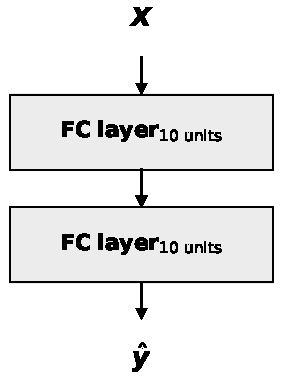
\includegraphics[width=0.293\columnwidth]{Figures/Diagrams/MLP.pdf}}
\caption{A multi-layer perceptron.}
\label{MLP} 
\end{figure}

\begin{figure}[H]
\centerline{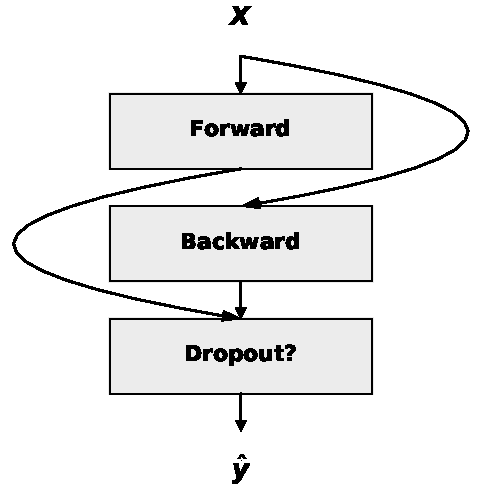
\includegraphics[width=0.5\columnwidth]{Figures/Diagrams/BD-LSTM.pdf}}
\caption{A bidirectional Long Short Term Memory network.}
\label{BD-LSTM}
\end{figure}

\begin{figure}[H]
\centerline{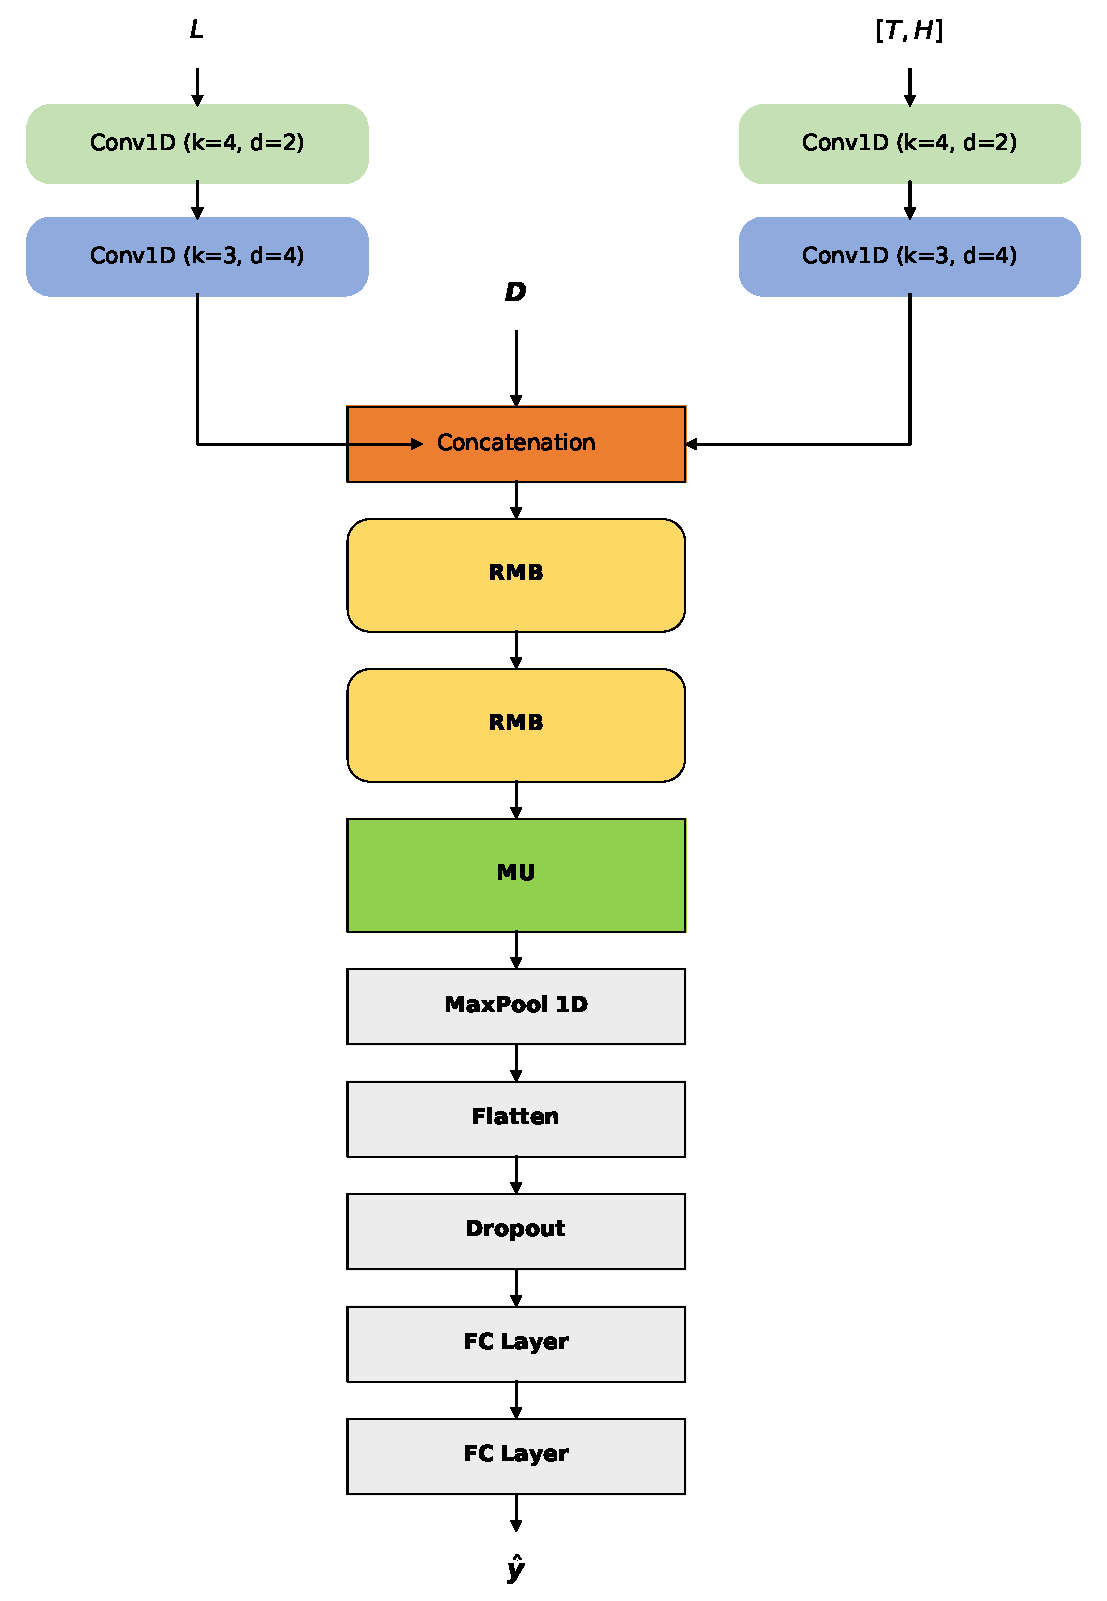
\includegraphics[width=0.9\columnwidth]{Figures/Diagrams/1D-CNN.pdf}}
\caption{A video-pixel-networks-based one-dimensional convolutional neural network. The input data are the load $L$, temperature $T$, hour of the day $H$, and a one-hot-encoding for the day of the week $\boldsymbol{D}$.}
\label{1D-CNN}
\end{figure}

\hypertarget{data}{\subsection{Data}\label{data}}

\renewcommand*\thetable{\arabic{table}} % Number tables starting at 1.
\CatchFileDef{\metadata}{Tables/metadata.tex}{} \metadata

\begin{figure}[H]
\centerline{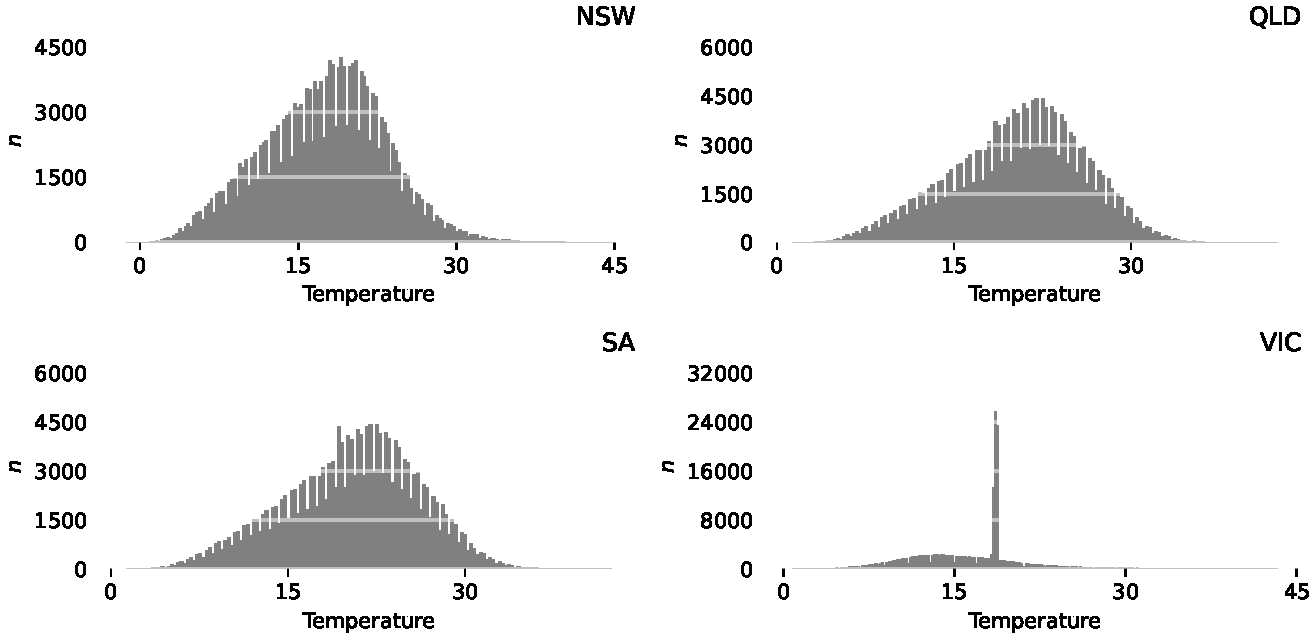
\includegraphics[width=0.8\columnwidth]{Figures/Plots/Temperature histogram.pdf}}
\caption{A histogram of the temperature data for NSW.}
\label{temp}
\end{figure}

\begin{figure}[H]
\centerline{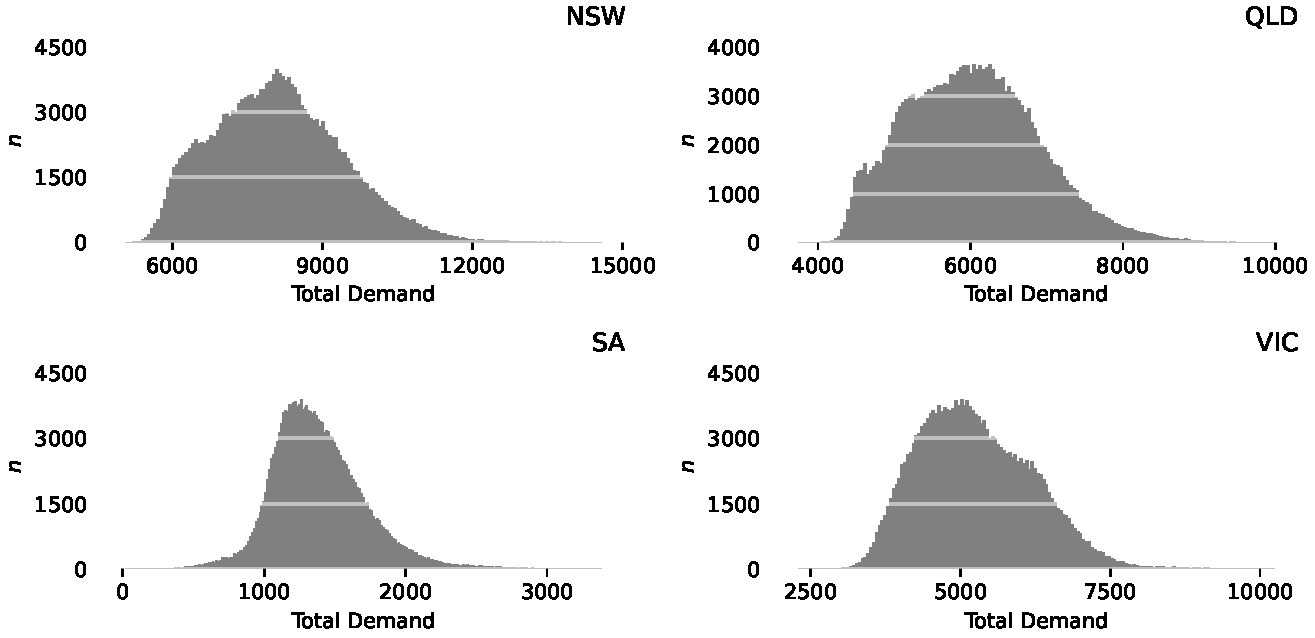
\includegraphics[width=0.8\columnwidth]{Figures/Plots/Total Demand histogram.pdf}}
\caption{A histogram of the total demand data for NSW.}
\label{tdemand}
\end{figure}

\begin{figure}[H]
\centerline{\includegraphics[width=0.8\columnwidth]{Figures/Plots/Total demand vs. temperature scatterplot.png}}
\caption{A scatter plot of total demand vs. temperature with a quadratic line of best fit.}
\label{temp_vs_tdemand}
\end{figure}

\begin{figure}[H]
\centerline{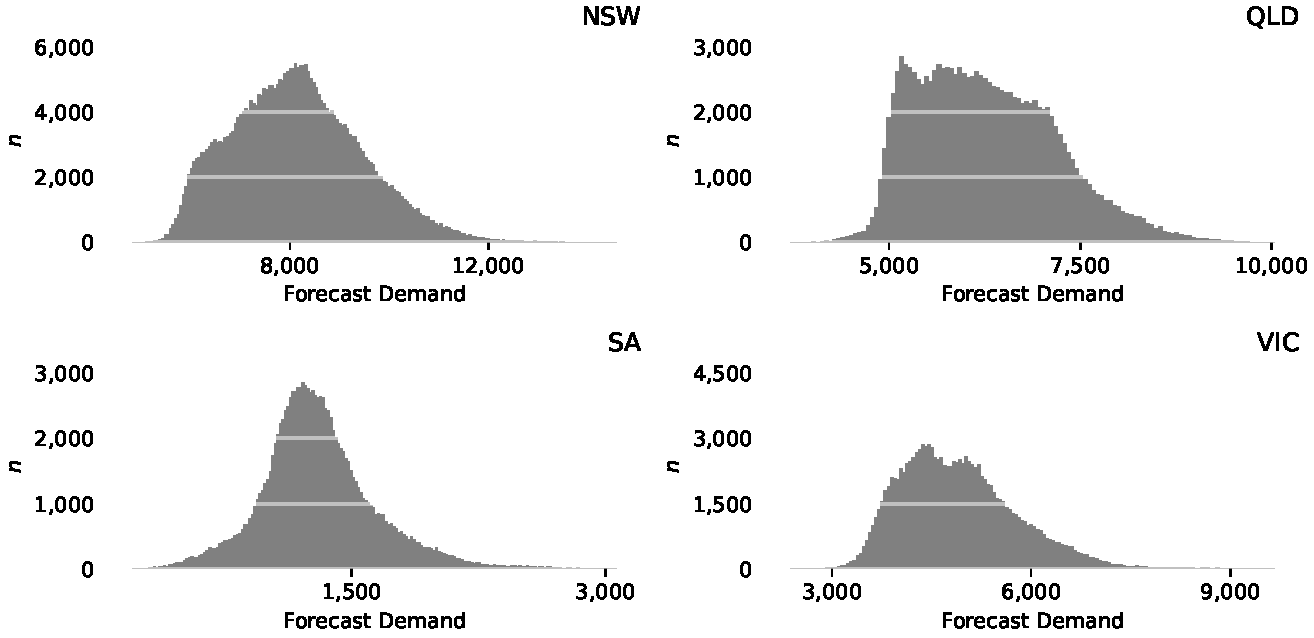
\includegraphics[width=0.8\columnwidth]{Figures/Plots/Forecast demand histogram.pdf}}
\caption{A histogram of forecasted demand for NSW.}
\label{fdemand}
\end{figure}

\begin{figure}[H]
\centerline{\includegraphics[width=\columnwidth]{Figures/Plots/Forecast vs. actual for 1- and 24-hours.png}}
\caption{Scatter plots of forecast vs. total demand for NSW. The one-hour-ahead (i.e. two-periods-ahead) correlation appears on the left, and the one-day-ahead correlation appears on the right.}
\label{fdemand_vs_tdemand}
\end{figure}

\begin{figure}[H]
\centerline{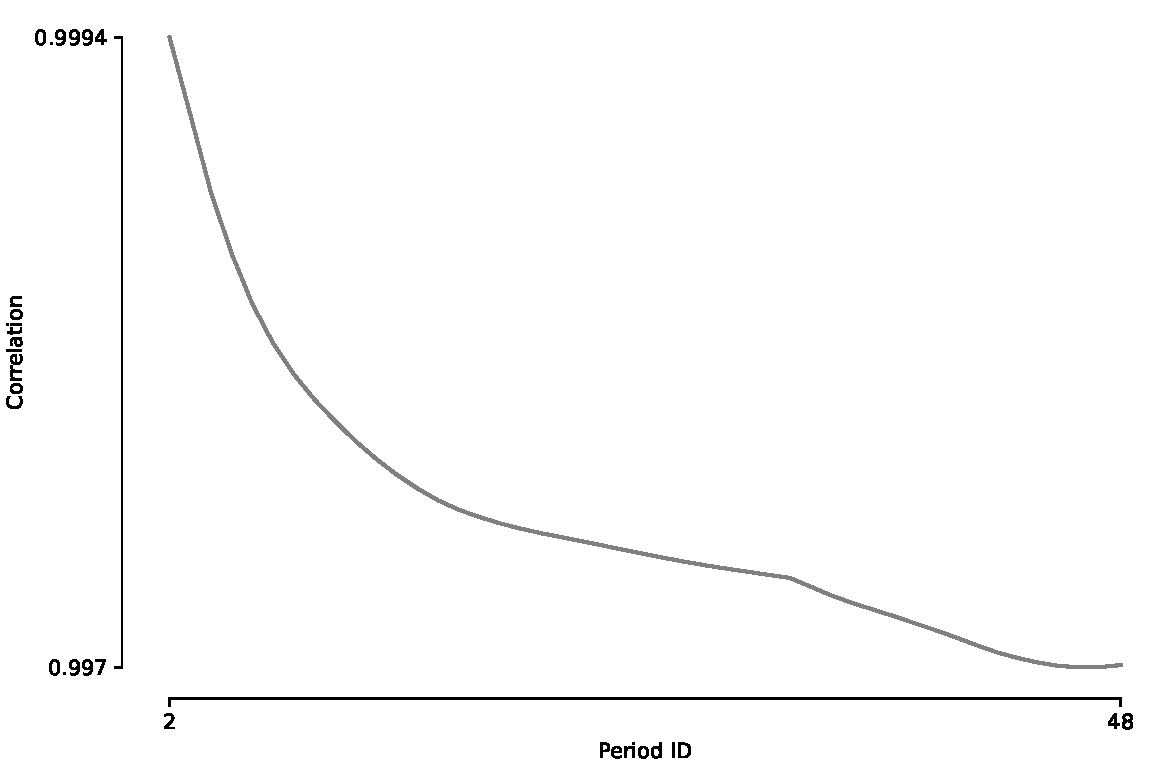
\includegraphics[width=0.8\columnwidth]{Figures/Plots/Forecast vs. actual correlation by Period ID.pdf}}
\caption{A line plot of the Pearson correlation coefficient of forecast and total demand vs. the period ID. Each period represents a thirty-minute interval. As such, the X-axis also represents the correlations from one-hour-ahead to one-day-ahead forecasts.}
\label{corr_by_per}
\end{figure}

\begin{figure}[H]
\centerline{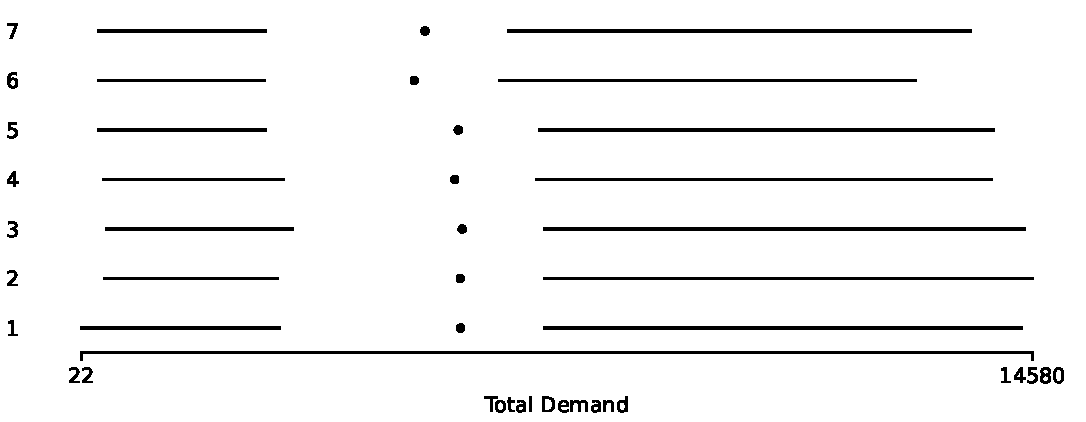
\includegraphics[width=0.8\columnwidth]{Figures/Plots/Demand by day boxplots.pdf}}
\caption{Tufte boxplots of total demand by day of the week. The data for each day are represented in quartiles, with lines for the first and fourth, whitespace for the second and third, and a dot at the median \cite{tufte}.}
\label{dem_by_day}
\end{figure}

\begin{figure}[H]
\centerline{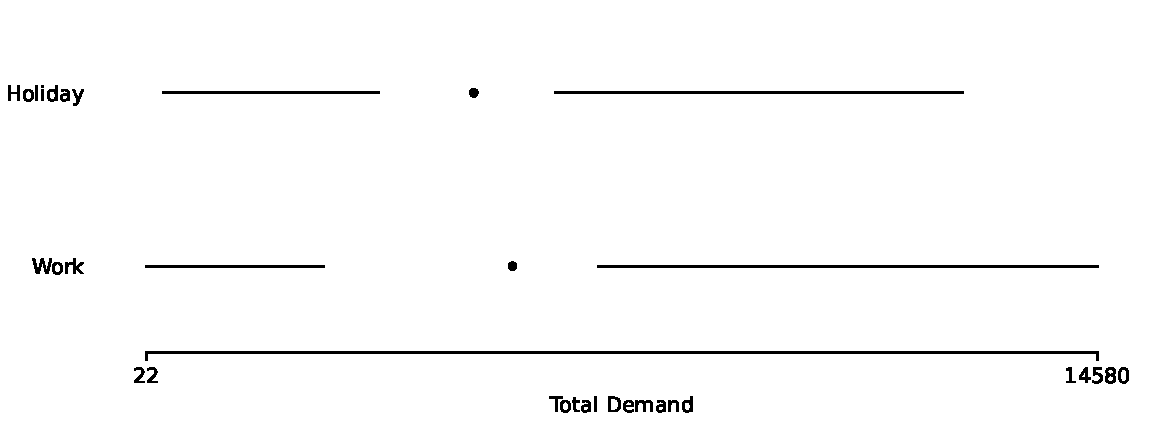
\includegraphics[width=0.8\columnwidth]{Figures/Plots/Demand by is-weekend boxplots.pdf}}
\caption{Tufte boxplots of total demand by is-weekend. The data for each day are represented in quartiles, with lines for the first and fourth, whitespace for the second and third, and a dot at the median \cite{tufte}.}
\label{is_weekend}
\end{figure}


\hypertarget{activities}{\subsection{Activities}\label{activities}}
\begin{landscape}
\begin{tabularx}{\linewidth}{@{} M{0.5cm} Y Y Y @{}}
\toprule
& \textbf{Discovery} & \textbf{Design} & \textbf{Delivery} \\
\midrule
\rotatebox[origin=c]{90}{\parbox{4.2cm}{\textbf{Project Governance}}} &
\begin{itemize}[leftmargin=*, nosep, after=\vspace{-1ex}, before=\vspace{-2.5ex}]
    \item Kick-off Meeting: Define scope, objectives.
    \item Resource Planning: Assign roles, software, dataset access.
\end{itemize} & 
\begin{itemize}[leftmargin=*, nosep, after=\vspace{-1.5ex}, before=\vspace{-2.5ex}]
    \item Set Communication Standards: Define meeting schedules, document protocols.

\end{itemize} &
\begin{itemize}[leftmargin=*, nosep, after=\vspace{-1.5ex}, before=\vspace{-2.5ex}]
    \item Update Meetings: Share progress, challenges, and solutions.
    \item Project Review: Assess project against goals and academic criteria.
\end{itemize} \\
\midrule
\rotatebox[origin=c]{90}{\parbox{8cm}{\textbf{Solution Delivery}}} & 
\begin{itemize}[leftmargin=*, nosep, after=\vspace{-1.5ex}, before=\vspace{-2.5ex}]
    \item Literature Review: Review academic papers on power demand prediction.
    \item Identify Additional Data Sources: Catalog available datasets, note limitations.
\end{itemize} &
\begin{itemize}[leftmargin=*, nosep, after=\vspace{-1.5ex}, before=\vspace{-2.5ex}]
    \item Data Analysis and Exploration: Visualize data to identify patterns.
    \item Clean and Pre-process Data: Normalize temperatures, encode time features.
    \item Feature Engineering: Create new features, select relevant ones.
    \item Model Architecture: Evaluate neural network types for suitability.
    \item Initial Coding: Setup data pipeline, model skeleton.
\end{itemize} &
\begin{itemize}[leftmargin=*, nosep, after=\vspace{-1.5ex}, before=\vspace{-2.5ex}]
    \item Model Training: Adjust learning rate, epochs.
    \item Hyper-parameter Tuning: Use grid search or random search.
    \item Evaluate Model: Employ cross-validation, calculate metrics (MAE, RMSE, R²).
    \item Documentation: Detail experimental setup, pre-processing steps, model choice.
    \item Prepare for delivery: Ready model for demonstration.
    \item Report Writing: Summarize methodology, findings, insights.
    \item Presentation Preparation: Develop narrative, create visuals for presentation.
\end{itemize} \\
\bottomrule
\end{tabularx}\newline

\hypertarget{timeline}{\subsection{Timeline}\label{timeline}}
\begin{ganttchart}[
    vgrid={*{6}{draw=none}, dotted}, % 7-day week with a dotted line to mark weeks
    hgrid,
    time slot format=isodate,
    x unit=0.325cm, % Adjust the width of each day
    y unit title=0.7cm,
    y unit chart=0.6cm,
    title/.style={fill=blue!20, draw=none, text=black},
    title label font=\scriptsize,
    bar/.style={fill=blue!50},
    bar label font=\normalsize,
    group/.style={draw=black, fill=green!30},
    group right shift=0,
    group top shift=.6,
    group height=.3,
    group peaks tip position=0,
    milestone/.style={fill=orange!75!black, rounded corners=3pt, draw=black},
    milestone label font=\normalsize\color{black}
    ]{2024-03-04}{2024-04-29}

    % Phase Labels
    \gantttitle{Discover}{14}
    \gantttitle{Design}{21}
    \gantttitle{Deliver}{21} \\
    
    % Week labels
    \gantttitle{O-Week}{7}
    \gantttitle{Week 1}{7}
    \gantttitle{Week 2}{7}
    \gantttitle{Week 3}{7}
    \gantttitle{Week 4}{7}
    \gantttitle{Week 5}{7}
    \gantttitle{Week 6}{7}
    \gantttitle{Week 7}{7} \\

    % Date labels
    \gantttitle{04/03 - 10/03}{7}
    \gantttitle{11/03 - 17/03}{7}
    \gantttitle{18/03 - 24/03}{7}
    \gantttitle{25/03 - 31/03}{7}
    \gantttitle{01/04 - 07/04}{7}
    \gantttitle{08/04 - 14/04}{7}
    \gantttitle{15/04 - 21/04}{7}
    \gantttitle{22/04 - 28/04}{7} \\
    
    % Project Governance Stream
    \ganttgroup{Project Governance}{2024-03-04}{2024-04-29} \\
    
    \ganttmilestone{Kick-off Meeting}{2024-03-08} \\
    
    \ganttmilestone{Leadership Meeting}{2024-03-11}
    \ganttmilestone{}{2024-03-18}
    \ganttmilestone{}{2024-03-25}
    \ganttmilestone{}{2024-04-01}
    \ganttmilestone{}{2024-04-08}
    \ganttmilestone{}{2024-04-15} \\
    
    \ganttmilestone{Weekly Team Meeting}{2024-03-15}
    \ganttmilestone{}{2024-03-22}
    \ganttmilestone{}{2024-03-29}
    \ganttmilestone{}{2024-04-05}
    \ganttmilestone{}{2024-04-12}
    \ganttmilestone{}{2024-04-19} \\
    
    \ganttmilestone{Weekly Task Planning}{2024-03-08}{2024-03-08}
    \ganttmilestone{}{2024-03-15}
    \ganttmilestone{}{2024-03-22}
    \ganttmilestone{}{2024-03-29}
    \ganttmilestone{}{2024-04-05}
    \ganttmilestone{}{2024-04-12}
    \ganttmilestone{}{2024-04-19} \\
    
    \ganttmilestone{Minutes Consolidation}{2024-03-09}
    \ganttmilestone{}{2024-03-16}
    \ganttmilestone{}{2024-03-23}
    \ganttmilestone{}{2024-03-30}
    \ganttmilestone{}{2024-04-06}
    \ganttmilestone{}{2024-04-13}
    \ganttmilestone{}{2024-04-20} \\
    
    \ganttmilestone{Project Review Meeting}{2024-04-22}{2024-04-22} \\
    
    % Solution Delivery Stream
    \ganttgroup{Solution Delivery}{2024-03-04}{2024-04-29} \\
    \ganttbar{Additional Source Identification}{2024-03-04}{2024-03-17} \\
    \ganttbar{Literature Review}{2024-03-04}{2024-03-22} \\
    \ganttbar{Model Architecture Selection}{2024-03-10}{2024-03-25} \\
    \ganttbar{Data Exploration}{2024-03-10}{2024-03-24} \\
    \ganttbar{Data Cleaning}{2024-03-18}{2024-03-31} \\
    \ganttbar{Feature Engineering}{2024-03-18}{2024-04-07} \\
    \ganttbar{Model Training \& Evaluation}{2024-03-25}{2024-04-20} \\
    \ganttbar{Report Writing}{2024-03-25}{2024-04-20} \\
    \ganttbar{Presentation Preparation}{2024-04-07}{2024-04-24}
\end{ganttchart}
\end{landscape}

\end{document}


